\documentclass[a4paper, 11pt]{article}

\usepackage[utf8]{inputenc}
\usepackage{babel}
\usepackage{hyperref}
\usepackage[capitalise, noabbrev]{cleveref}
\usepackage{a4wide}
\usepackage{graphicx}
\usepackage{float}
\usepackage{relsize}
\usepackage{indentfirst}
\usepackage{nameref}
\usepackage{listings}
\usepackage[newfloat]{minted}
\usepackage{caption}
\usepackage[normalem]{ulem}
\usepackage{setspace}
\usepackage[toc, page]{appendix}

\onehalfspacing

\hypersetup{
    pdftitle={Big Data \& Cloud Computing - 1st Practical Assignment},
    pdfborder={0 0 0}
}

\newenvironment{code}{\captionsetup{type=listing}}{}

\AtBeginEnvironment{minted}{\let\itshape\relax}

\title{Big Data \& Cloud Computing \\ [0.8em] \smaller 1\textsuperscript{st} Practical Assignment}
\author{David Capela \and Rui Fernandes}
\date{\today}

\begin{document}

\renewcommand\labelitemi{--}
\renewcommand{\today}{\ifcase \month\or January\or February\or March\or %
April\or May\or June\or July\or August\or September\or October\or November\or %
December\fi, \number \year}

\begin{titlepage}
    \begin{center}
        \begin{minipage}{.75\linewidth}
            \centering
            
\includegraphics[width=0.5\textwidth]{img/fcup.jpg}\par\vspace{1cm}
            \vspace{1.5cm}
            {\scshape\LARGE Faculty of Sciences of the University of Porto} \par
            \vspace{1cm}
            {\scshape\Large Master's Degree in Information Security} \par
            \vspace{1.5cm}
            \maketitle
        \end{minipage}
    \end{center}
    \vspace{2cm}
    \thispagestyle{empty}
    \pagebreak
\end{titlepage}

\pagenumbering{roman}

\begin{abstract}
This report describes the first practical assignment of the Big Data \& Cloud Computing course of 
the Master's Degree in Information Security at the Faculty of Sciences of the University of Porto.

This assignment aims at developing an AppEngine app that not only provides information about images 
taken from the Open Images dataset, but also employs a TensorFlow model for image classification 
derived using AutoML Vision.

In this report, we briefly describe the application we developed and discuss the decisions we made. 
\end{abstract}

\pagebreak

\tableofcontents
\listoffigures 
\lstlistoflistings

\pagebreak

\pagenumbering{arabic}

\section{Introduction}

This project consists in developing an AppEngine app that provides information about images from 
the Open Images dataset. In addition, the app makes use of a TensorFlow model for image 
classification derived from AutoML Vision. As such, the work is divided into the following parts:

\begin{enumerate}
    \item Defining a BigQuery dataset from CSV files.
    \item Implementing the app endpoints to query data stored in BigQuery, and reference the 
    corresponding image files stored in a public storage bucket.
    \item Deriving our own TensorFlow model with AutoML, which replaces the one provided with the 
    application.
    \item Developing an endpoint for image classification that uses label detection through the 
    Google Cloud Vision API.
    \item Defining our own Docker container for the app.
\end{enumerate}

\begin{table}[H]
\centering
\begin{tabular}{|c|c|}
\hline
\textbf{Project ID}     & \texttt{big-data-project1-347618} \\ \hline
\textbf{AppEngine URL} & \url{https://big-data-project1-347618.uc.r.appspot.com} \\ \hline
\textbf{Docker container URL on Cloud Run}   & \url{https://demo-app-uqhmrwookq-oa.a.run.app} \\ \hline
\end{tabular}
\end{table}

\vspace{\baselineskip}

\subsection*{Structure of the Report}

The remainder of this work is structured as follows:

\begin{itemize}
    \item In \cref{sec:data-model}, \textbf{\nameref{sec:data-model}}, we describe the data model,
    the available endpoints and how they were implemented.
    \item In \cref{sec:tensorflow}, \textbf{\nameref{sec:tensorflow}}, we explain how we our own 
    TensorFlow model with AutoML, replacing the one provided with the application.
    \item In \cref{sec:aditional-challenges}, \textbf{\nameref{sec:aditional-challenges}}, the 
    additional challenges are addressed, which include image classification through the Google Cloud 
    Vision API, and defining a Docker container for the app.
    \item Finally, \cref{sec:conclusion}, \textbf{\nameref{sec:conclusion}}, concludes the report.
\end{itemize}

\pagebreak

\section{Data Model \& Application Endpoints} \label{sec:data-model}

The BigQuery dataset contains the following three tables:

\begin{itemize}
    \item \texttt{classes}: Contains the label and a brief description of each 
    \item \texttt{image\_labels}: Contains the image ID and the respective class label.
    \item \texttt{relations}: Contains the image ID, and the relationship between the respective 
    classes.
\end{itemize}

This data model is illustrated in \cref{fig:data-model}.

\vspace{\baselineskip}

\begin{figure}[H]
    \centering
    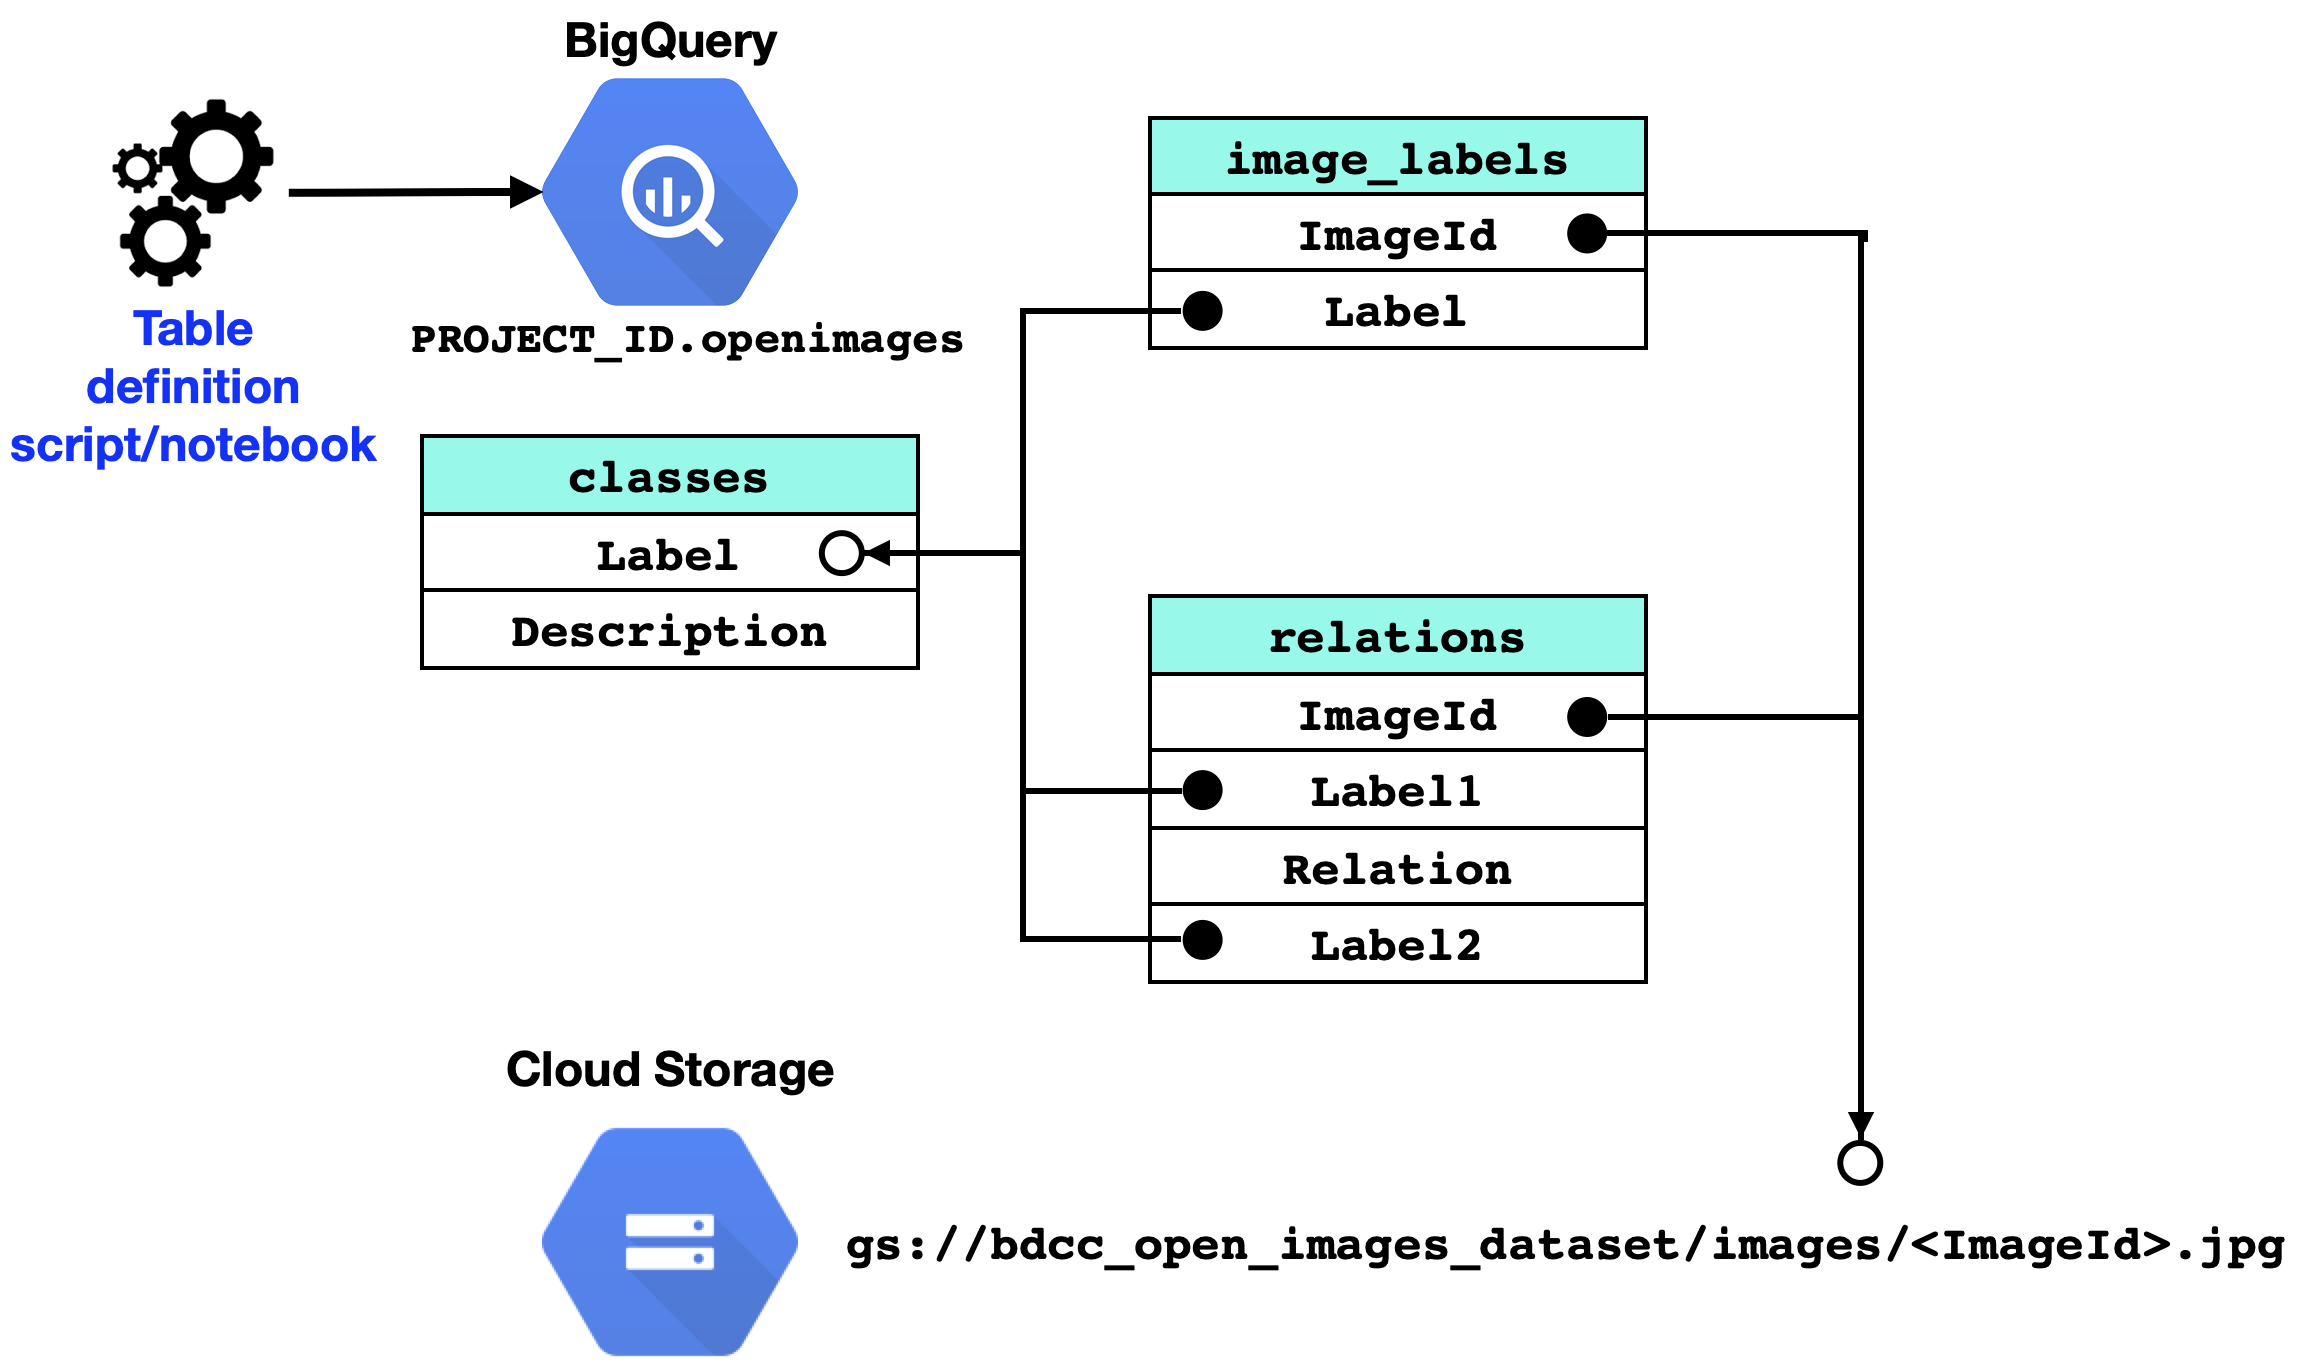
\includegraphics[width=.75\textwidth]{img/data-model.png}
    \caption{Data model}
    \label{fig:data-model}
\end{figure}

For initial development of the app, we used the \texttt{bdcc22project.openimages} BigQuery dataset. 
However, we then defined our own BigQuery data set. To do so, we wrote a Python script, as shown in 

To access information contained in the dataset, a few endpoints were implemented. Each endpoint 
performs one or more BigQuery queries, and the returned data is used to create an HTML page that 
displays such data to the user.

The following application endpoints were already implemented:

\begin{itemize}
    \item \texttt{classes}: List image labels.
    \item \texttt{image\_search}: Search for images based on a single label.	
    \item \texttt{image\_classify\_classes}: List available classes for image classification.	
    \item \texttt{image\_classify}: Use a TensorFlow model to classify images.	
\end{itemize}

This being said, we only had to implement the following endpoints:

\begin{itemize}
    \item \texttt{image\_info}: Get information for a single image.
    \item \texttt{relations}: List relation types.
    \item \texttt{relations\_search}: Search for images by relation.
    \item \texttt{image\_search\_multiple}: Search for images based on multiple labels.
\end{itemize}

The implementation of these endpoints is described in detail in the following sections, and 
snippets of code are included.

\subsection{Image Info Endpoint}

This endpoint lists information about a single image, \textit{i.e.} a list of all relations and 
classes, given its ID. To do so, we wrote two queries: the first one selects the classes by joining 
the \texttt{image\_labels} and \texttt{classes} tables using the label and filtering by those that 
have the requested ID. By doing so, we end up with the description of all the classes of the image 
in question.

In addition, the second query selects existing relationships between between any two classes by 
joining the \texttt{relations} and \texttt{classes} tables and then filtering by those that have 
the requested ID.

Having said this, the implementation of this endpoint is shown in \cref{code:image_info}.

\subsection{Relations Endpoint}

This endpoint returns the relations between images. To do so, the query selects all relations, 
counts the number of images that satisfy each relation, groups them, and, finally, sorts them 
alphabetically. Thus, we end up with the number of images that satisfy each relation.

The implementation of this endpoint is shown in \cref{code:relations}.

\subsection{Relation Search Endpoint}

This endpoint search for images that satisfy a given relation (\textit{e.g. Man holds Guitar}, 
where \textit{Man} and \textit{Guitar} are the classes and \textit{holds} is the relation between 
them). In this case, the classes can be specified or default (denoted with the symbol \texttt{\%}), 
and the limit of images to be displayed can also be specified.

To do so, the query selects \texttt{ImageId}, \texttt{Class1}, \texttt{Relation} and 
\texttt{Class2} by joining the \texttt{relations} the \texttt{classes} tables when the relations 
and the classes are the ones specified.

It is worth noting that this query makes use of the \texttt{LIKE} SQL operator such that, if no 
class parameters are supplied, the query uses the default \texttt{\%}, returning image that 
satisfies the relationship, regardless of the classes involved in it.

The implementation of this endpoint is shown in \cref{code:relation_search}.

\subsection{Image Search Multiple Endpoint}

This query selects all images that correspond to at least one of the classes specified by the user, 
as well as the number of classes that matched. This search is performed in the 
\texttt{image\_labels} table, as well as the classes table, using the \texttt{Label} attribute. To 
do so, we use two different functions:

\begin{itemize}
    \item \texttt{ARRAY\_AGG} is used to return an array with the classes associated with the said 
    image.
    \item \texttt{UNNEST} is used to to transform the previously mentioned array in order to check 
    whether a description was contained in the values of that same table.
\end{itemize}

The implementation of this endpoint is shown in \cref{code:image_search_multiple}.

\pagebreak

\section{TensorFlow Model Using AutoML} \label{sec:tensorflow}

We started by creating an AutoML dataset using a Python script \texttt{copy\_images.py} that copied 
relevant bucket images from the provided example bucket to ours. After having the images in our 
bucket, we had to generate the \texttt{automl.csv} file that stated the images we wanted the AutoML 
model to be trained with and for that we used the \texttt{create\_automl.py} script.
Finally, we uploaded the result file from the last script into the AutoML project in Google Cloud 
and waited for it to be finished so we could download the \texttt{tflite.model} file. This process 
is illustrated in \cref{fig:auto-ml}.

\vspace{\baselineskip}

\begin{figure}[H]
    \centering
    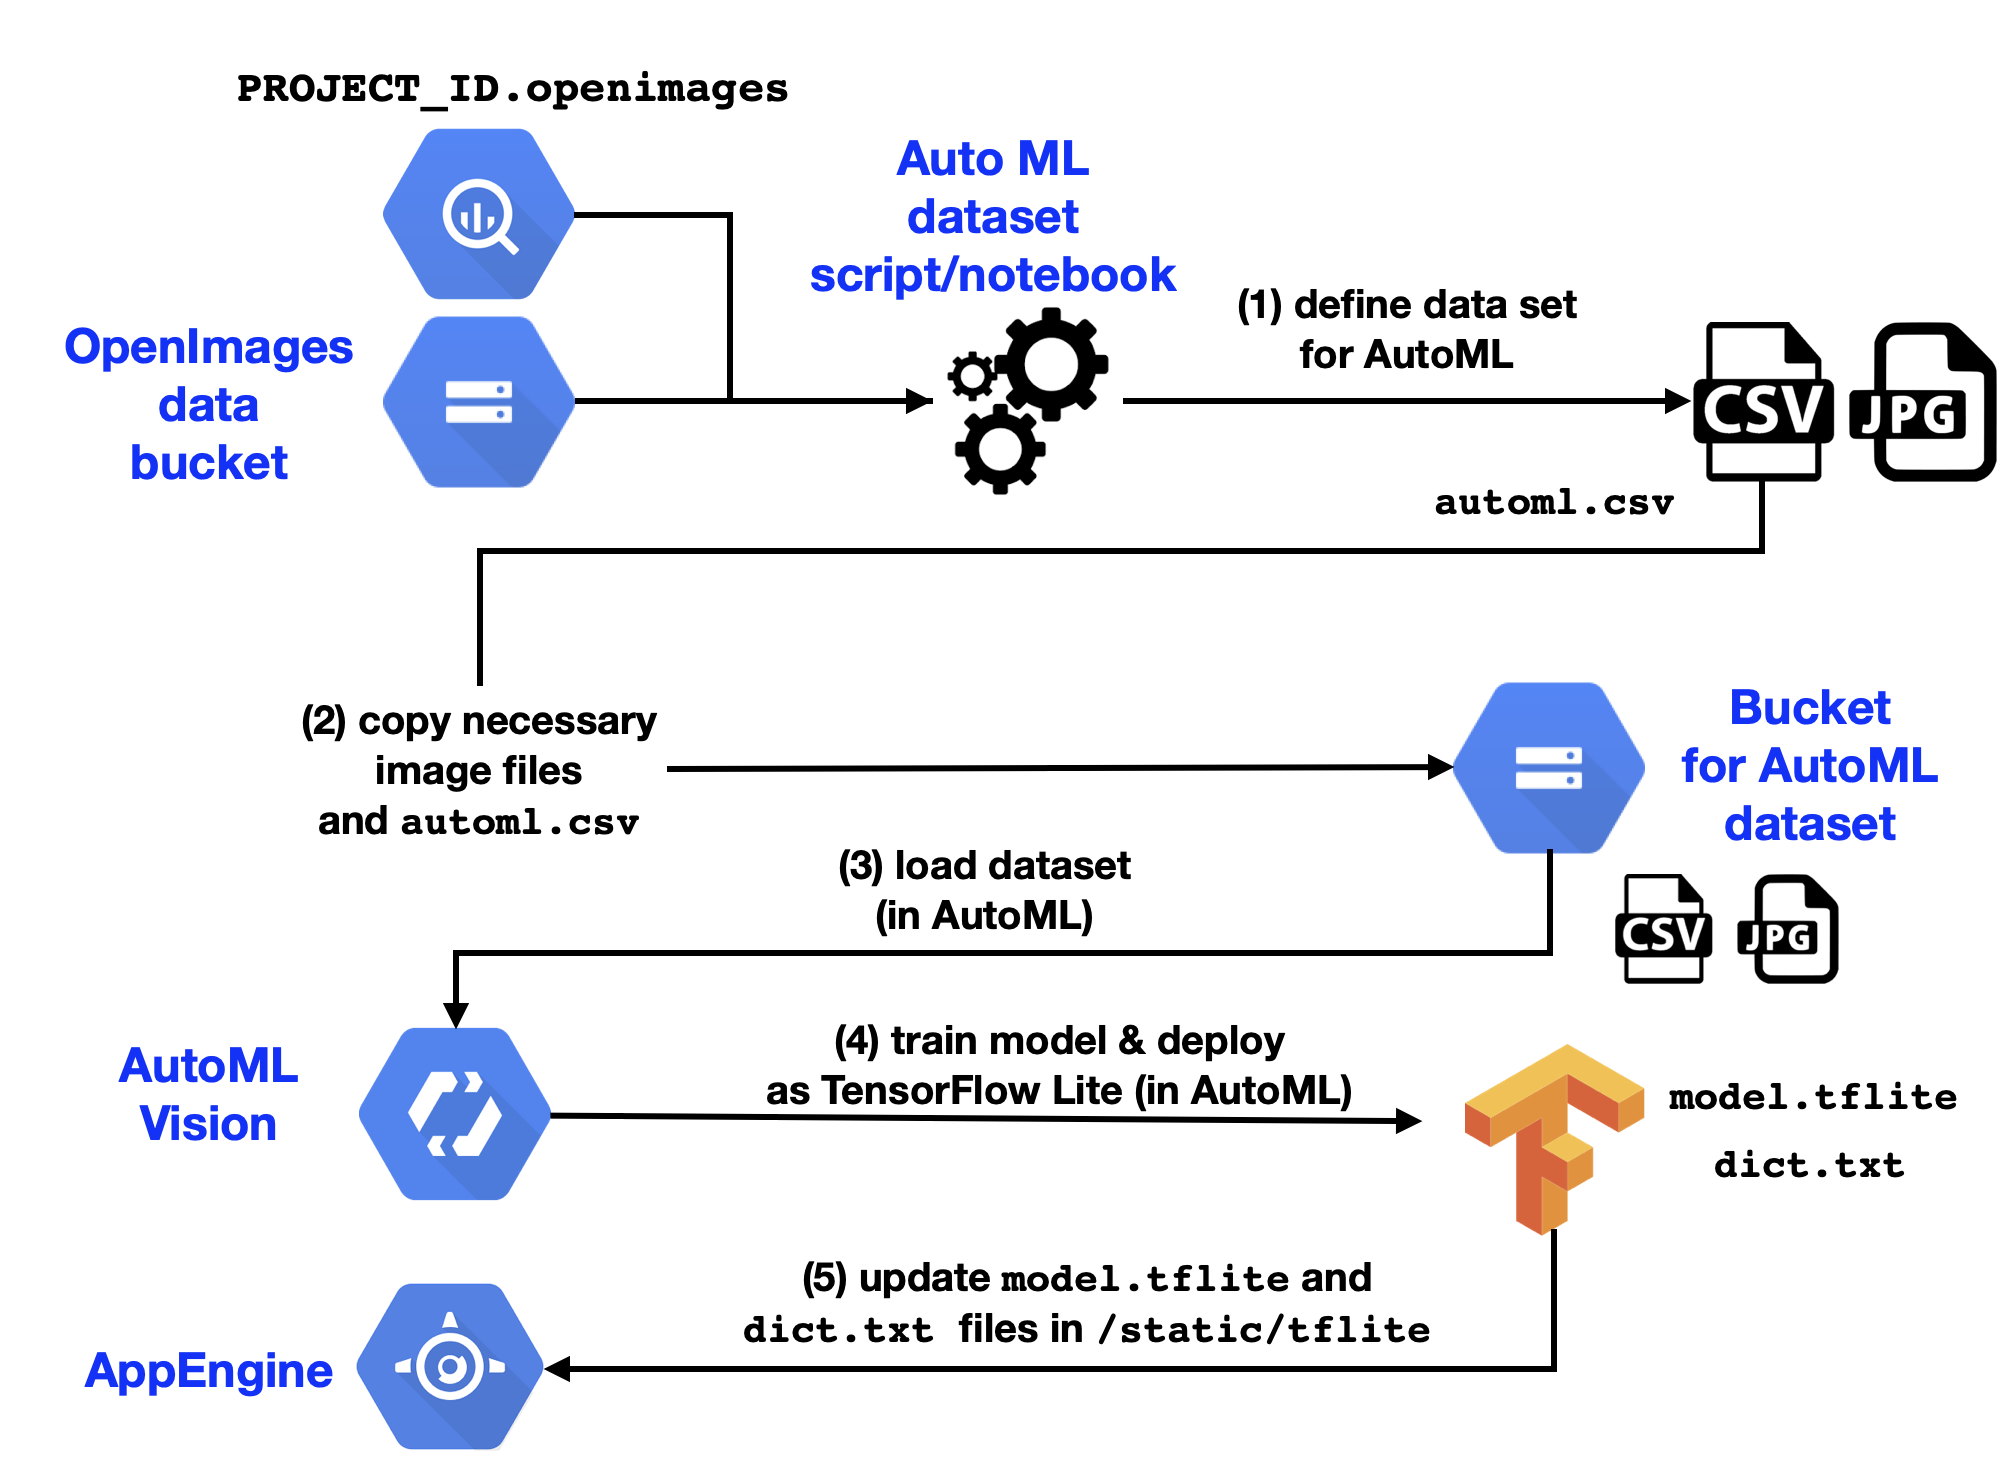
\includegraphics[width=.85\textwidth]{img/automl.png}
    \caption{TensorFlow model to classify images}
    \label{fig:auto-ml}
\end{figure}

\pagebreak

\section{Additional Challenges} \label{sec:aditional-challenges}

In this section, we address the additional challenges, namely the implementation of an alternative 
endpoint for image classification using label detection through the Google Cloud Vision API, and 
the necessary steps we took in order to define our own Docker container for the application.

\subsection{Label Detection Using Cloud Vision API}

Besides creating our own TensorFlow model to perform image classification, we also implemented an 
endpoint that detects image labels by using Google's Cloud Vision API. The implementation of this 
endpoint can be seen in \cref{code:cloud_vision}.

\subsection{Docker Image}

Before defining the Docker container, we have to change \texttt{host='127.0.0.1'} to 
\texttt{host='0.0.0.0'} in the main function, that is, the \texttt{main} function is as follows:

\begin{minted}{py}
if __name__ == '__main__':
    # When invoked as a program.
    logging.info('Starting app')
    app.run(host='0.0.0.0', port=8080, debug=True)
\end{minted}

This happens because the web server running in the container is listening for connections on port 
\texttt{8080} of the loopback network interface (\texttt{127.0.0.1}). Thus, it will only respond to 
HTTP requests originating from the container itself. To accept connections from outside of the 
container, we have to bind it to the \texttt{0.0.0.0} IP address.

Another thing to keep in mind is that we have to specify the \texttt{GOOGLE\_CLOUD\_PROJECT} 
environment variable, otherwise the project ID cannot be determined. This being said, the 
Dockerfile is as follows:

\vspace{\baselineskip}

\begin{code}
\begin{minted}{py}
# Python image to use.
FROM python:3.8

# Set the working directory to /app
WORKDIR /app

# Copy the requirements file used for dependencies
COPY requirements.txt .

# Install any needed packages specified in requirements.txt
RUN pip install --trusted-host pypi.python.org -r requirements.txt

# Copy the rest of the working directory contents into the container at /app
COPY . .

# Set the GOOGLE_CLOUD_PROJECT environment variable
ENV GOOGLE_CLOUD_PROJECT=big-data-project1-347618

# Define network ports for the container to listen on at runtime
EXPOSE 8080

# Run main.py when the container launches
ENTRYPOINT ["python", "main.py"]
\end{minted}
\captionof{listing}{Dockerfile}
\label{code:dockerfile}
\end{code}

\vspace{\baselineskip}

We can run the app using Docker with the following commands:

\begin{verbatim}
$ docker build -t bdcc22 .
$ docker run -d -p 8080:8080 bdcc22
\end{verbatim}

Finally, the application was deployed using Google Cloud Run, an is now available at 
\url{https://demo-app-uqhmrwookq-oa.a.run.app}. However, it is worth noting that sometimes we get a 
"Service Unavailable" error when we try to access the web page. After trying different region 
parameters (namely, \texttt{europe-west1}, \texttt{europe-west6} and \texttt{us-central1}), the 
error remained, and due to time constraints, we were not able to look further into this issue. 
Regardless, given the fact that we can run the application with the command \texttt{docker run -d 
-p 8080:8080 bdcc22}, we know that the Dockerfile is well defined.

\pagebreak

\section{Conclusions} \label{sec:conclusion}

This project has been extremely valuable in terms of understanding the theoretical concepts taught 
in class, its challenges, and how they can be applied to real-world applications using big data and 
cloud computing.

As a matter of fact, we were able to implement all of the endpoints and create our own TensorFlow 
model
with AutoML Vision, which allows us to perform image classification.

\pagebreak

\begin{appendix}

\section{Image Info Endpoint}

\begin{code}
\begin{minted}{py}
@app.route('/image_info')
def image_info():
    image_id = flask.request.args.get('image_id')

    results_classes = BQ_CLIENT.query(
        '''
        SELECT Description
        FROM `big-data-project1-347618.dataset1.labels`
        JOIN `big-data-project1-347618.dataset1.classes` USING(label)
        WHERE ImageId = '{0}'
        ORDER BY Description ASC
    '''.format(image_id)
    ).result()

    results_relations = BQ_CLIENT.query(
        '''
        SELECT C1.Description as Class1, R.Relation, C2.Description as Class2
        FROM `big-data-project1-347618.dataset1.relations` R
        JOIN `big-data-project1-347618.dataset1.classes` C1 ON (R.label1=C1.label)
        JOIN `big-data-project1-347618.dataset1.classes` C2 ON (R.label2=C2.label)
        WHERE R.ImageId = '{0}'
    '''.format(image_id)
    ).result()

    data = dict(description=image_id,
                classes=results_classes,
                relations=results_relations
                )
    logging.info('image_info: image_id={}, classes={}, relations={}'.format(
        image_id, results_classes.total_rows, results_relations.total_rows))
    return flask.render_template('image_id.html', data=data)

\end{minted}
\captionof{listing}{Implementation of the \texttt{image\_info} endpoint}
\label{code:image_info}
\end{code}

\pagebreak

\section{Relations Endpoint}

\hspace{0pt}
\vfill

\begin{code}
\begin{minted}{py}
@app.route('/relations')
def relations():
    results = BQ_CLIENT.query(
        '''
        SELECT Relation, COUNT(*) As NumImages
        FROM `big-data-project1-347618.dataset1.relations`
        GROUP BY Relation
        ORDER BY Relation ASC
    ''').result()

    logging.info('classes: results={}'.format(results.total_rows))
    
    data = dict(results=results)
    
    return flask.render_template('relations.html', data=data)
\end{minted}
\captionof{listing}{Implementation of the \texttt{relations} endpoint}
\label{code:relations}
\end{code}

\vfill
\hspace{0pt}

\pagebreak

\section{Relation Search Endpoint}

\begin{code}
\begin{minted}{py}
@app.route('/relation_search')
def relation_search():
    class1 = flask.request.args.get('class1', default='%')
    relation = flask.request.args.get('relation', default='%')
    class2 = flask.request.args.get('class2', default='%')
    image_limit = flask.request.args.get('image_limit', default=10, type=int)

    results = BQ_CLIENT.query(
        '''
        SELECT R.ImageId, C1.Description as Class1, R.Relation, C2.Description as Class2
        FROM `big-data-project1-347618.dataset1.relations` R
        JOIN `big-data-project1-347618.dataset1.classes` C1 ON (R.label1=C1.label)
        JOIN `big-data-project1-347618.dataset1.classes` C2 ON (R.label2=C2.label)
        WHERE R.Relation LIKE '{0}'
        AND C1.Description LIKE '{1}'
        AND C2.Description LIKE '{2}'
        ORDER BY R.ImageId
        LIMIT {3}
    '''.format(relation, class1, class2, image_limit)
    ).result()

    logging.info('relation_search: limit={}, results={}'
                 .format(image_limit, results.total_rows))
    data = dict(class1=class1,
                class2=class2,
                relation=relation,
                image_limit=image_limit,
                results=results)
    return flask.render_template('relation_search.html', data=data)
\end{minted}
\captionof{listing}{Implementation of the \texttt{relation\_search} endpoint}
\label{code:relation_search}
\end{code}

\pagebreak

\section{Image Search Multiple Endpoint}

\begin{code}
\begin{minted}{py}
@app.route('/image_search_multiple')
def image_search_multiple():
    descriptions = flask.request.args.get('descriptions').split(',')
    image_limit = flask.request.args.get('image_limit', default=10, type=int)

    results = BQ_CLIENT.query(
        '''
        SELECT ImageId, ARRAY_AGG(Description), COUNT(Description)
        FROM big-data-project1-347618.dataset1.labels
        JOIN big-data-project1-347618.dataset1.classes USING(label)
        WHERE Description IN UNNEST({0})
        GROUP BY ImageId
        ORDER BY Count(Description) DESC, ImageId
        LIMIT {1}
    '''.format(descriptions, image_limit)
    ).result()

    logging.info(
        'image_search_multiple: descriptions={} image_limit={} results={}'.format(
            descriptions, image_limit, results.total_rows)
    )
    data = dict(descriptions=descriptions,
                image_limit=image_limit,
                results=results)
    return flask.render_template(
        'image_search_multiple.html',
        data=data,
        descriptions=descriptions,
        image_limit=image_limit,
        total=results.total_rows,
        description_len=len(descriptions)
    )
\end{minted}
\captionof{listing}{Implementation of the \texttt{image\_search\_multiple} endpoint}
\label{code:image_search_multiple}
\end{code}

\pagebreak

\section{Label Detection Using Cloud Vision API}

\begin{code}
\begin{minted}{py}
@app.route('/cloud_vision', methods=['POST'])
def cloud_vision():
    files = flask.request.files.getlist('files')
    min_confidence = 1

    results = []
    if len(files) > 1 or files[0].filename != '':
        for file in files:
            blob = storage.Blob(file.filename, APP_BUCKET)
            blob.upload_from_file(file, blob, content_type=file.mimetype)

            client = vision.ImageAnnotatorClient()
            image = vision.Image()
            image.source.image_uri = 'https://storage.googleapis.com/' + \
                APP_BUCKET.name + '/' + file.filename

            response = client.label_detection(image=image)

            if response.error.message:
                raise Exception(
                    '{}\nFor more info on error messages, check: '
                    'https://cloud.google.com/apis/design/errors'.format(
                        response.error.message
                    )
                )

            classifications = response.label_annotations
            scores = list(map(lambda x: x.score, classifications))

            if min(scores) < min_confidence:
                min_confidence = min(scores)

            logging.info('cloud_vision: filename={} blob={} classifications={}, scores={}'
                         .format(file.filename, blob.name, classifications, scores))
            results.append(dict(bucket=APP_BUCKET,
                                filename=file.filename,
                                classifications=classifications))

    data = dict(bucket_name=APP_BUCKET.name,
                min_confidence='{:.5f}'.format(min_confidence),
                results=results)
    return flask.render_template('cloud_vision.html', data=data)
\end{minted}
\captionof{listing}{Implementation of the \texttt{cloud\_vision} endpoint}
\label{code:cloud_vision}
\end{code}

\end{appendix}

\end{document}
